%%%%%%%%%%%%%%%%%%%%%%%%%%%%%%%%%%%%%%%%%
% baposter Landscape Poster
% LaTeX Template
% Version 1.0 (11/06/13)
%
% baposter Class Created by:
% Brian Amberg (baposter@brian-amberg.de)
%
% This template has been downloaded from:
% http://www.LaTeXTemplates.com
%
% License:
% CC BY-NC-SA 3.0 (http://creativecommons.org/licenses/by-nc-sa/3.0/)
%
%%%%%%%%%%%%%%%%%%%%%%%%%%%%%%%%%%%%%%%%%

%----------------------------------------------------------------------------------------
%	PACKAGES AND OTHER DOCUMENT CONFIGURATIONS
%----------------------------------------------------------------------------------------

\documentclass[landscape,a0paper,fontscale=0.285]{baposter} % Adjust the font scale/size here

\usepackage{graphicx} % Required for including images
\graphicspath{{figures/}} % Directory in which figures are stored

\usepackage{amsmath} % For typesetting math
\usepackage{amssymb} % Adds new symbols to be used in math mode

\usepackage{booktabs} % Top and bottom rules for tables
\usepackage{enumitem} % Used to reduce itemize/enumerate spacing
\usepackage{palatino} % Use the Palatino font
\usepackage[font=small,labelfont=bf]{caption} % Required for specifying captions to tables and figures

\usepackage{hyperref}
\usepackage{url}

\usepackage{multicol} % Required for multiple columns
\setlength{\columnsep}{1.5em} % Slightly increase the space between columns
\setlength{\columnseprule}{0mm} % No horizontal rule between columns

\usepackage{tikz} % Required for flow chart
\usetikzlibrary{shapes,arrows} % Tikz libraries required for the flow chart in the template

\newcommand{\compresslist}{ % Define a command to reduce spacing within itemize/enumerate environments, this is used right after \begin{itemize} or \begin{enumerate}
\setlength{\itemsep}{1pt}
\setlength{\parskip}{0pt}
\setlength{\parsep}{0pt}

}

\definecolor{lightblue}{rgb}{0.145,0.6666,1} % Defines the color used for content box headers

\begin{document}

\begin{poster}
{
headerborder=closed, % Adds a border around the header of content boxes
colspacing=1em, % Column spacing
bgColorOne=white, % Background color for the gradient on the left side of the poster
bgColorTwo=white, % Background color for the gradient on the right side of the poster
borderColor=lightblue, % Border color
headerColorOne=black, % Background color for the header in the content boxes (left side)
headerColorTwo=lightblue, % Background color for the header in the content boxes (right side)
headerFontColor=white, % Text color for the header text in the content boxes
boxColorOne=white, % Background color of the content boxes
textborder=roundedleft, % Format of the border around content boxes, can be: none, bars, coils, triangles, rectangle, rounded, roundedsmall, roundedright or faded
eyecatcher=true, % Set to false for ignoring the left logo in the title and move the title left
headerheight=0.1\textheight, % Height of the header
headershape=roundedright, % Specify the rounded corner in the content box headers, can be: rectangle, small-rounded, roundedright, roundedleft or rounded
headerfont=\Large\bf\textsc, % Large, bold and sans serif font in the headers of content boxes
%textfont={\setlength{\parindent}{1.5em}}, % Uncomment for paragraph indentation
linewidth=2pt % Width of the border lines around content boxes
}
%----------------------------------------------------------------------------------------
%	TITLE SECTION 
%----------------------------------------------------------------------------------------
%
{
\includegraphics[height=4em]{drexel.png}} % First university/lab logo on the left
{\bf\textsc{House in Your Head}\vspace{0.5em}} % Poster title
{\textsc{\{Samuel Bever, Michael Conway, Joseph Muoio, Kyle Patron, Kevin Zakszewski\} \hspace{12pt} Drexel University: CCI}} % Author names and institution
{
\includegraphics[height=4em]{logo.png}} % Second university/lab logo on the right

%----------------------------------------------------------------------------------------
%	OBJECTIVES
%----------------------------------------------------------------------------------------

\headerbox{Objectives}{name=objectives,column=0,row=0}{

The goal of this project is to cater to ALS patients, giving them the ability to be more autonomous. The key features are:

\begin{itemize}
\item Calibration for individual users
\item Intuitive interface with simple selections
\item Allow users with ALS to perform basic household tasks, such as
    \begin{itemize}
        \item Turning lights on and off
        \item Controlling the television
        \item Controlling a keyboard
    \end{itemize}
\end{itemize}

\vspace{0.3em} % When there are two boxes, some whitespace may need to be added if the one on the right has more content
}

%----------------------------------------------------------------------------------------
%	INTRODUCTION
%----------------------------------------------------------------------------------------

\headerbox{Introduction}{name=introduction,column=1,row=0, aligned=objectives}{

Amyotrophic lateral sclerosis (ALS, also called ``Lou Gehrig's Disease'') is
a neurodegenerative disease affecting the brain and spinal cord. The motor
neurons progressively degenerate and die off, leading to the loss of muscle
control and death. Affected individuals suffer a spectrum of symptoms
culminating in total lock-in. In this state, the patient is aware but cannot
move their muscles. Because of this, late-stage ALS patients are unable to interface
with conventional assistive technologies. \cite{ALSsource} \\

The goal of the project is to build a system which people afflicted with ALS
can use to interact with their houses through an Insteon Home Automation System (HAS) \cite{Insteon} and an Emotiv EEG reader \cite{Emotiv}.
This includes controlling devices like the lights, stereo, and
television. By having a Brain Computer Interface (BCI) to their automated
house, individuals with ALS can still interact with their environment despite
full paralysis.
}

%----------------------------------------------------------------------------------------
%	Architecture
%----------------------------------------------------------------------------------------

\headerbox{System Overview}{name=architecture,column=2,span=2,row=0}{

\begin{multicols}{2}
\vspace{1em}
\begin{center}
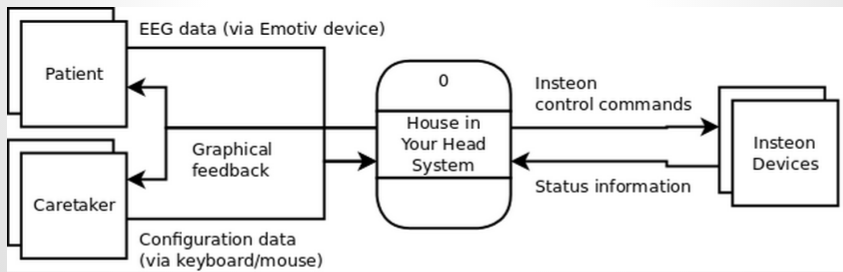
\includegraphics[width=0.8\linewidth]{contextDiagram}
\captionof{figure}{Context Diagram of the system}
\end{center}

The system is broken down into 3 main components: the graphical user interface
(GUI), electroencephalogram (EEG) processing, and the home automation system
(HAS). The GUI can be shown on any standard computer display. It scrolls
through options one by one until the user makes a selection by thinking their
``accepting thought,'' which the EEG processing component is trained to
recognize; recommended accepting thoughts include adding numbers, counting,
and mentally composing a letter to a friend.

The option that is displayed on the GUI at the time of the accept thought is
selected and the appropriate call to the HAS component is made. For instance,
if the option to turn on a light was shown in the GUI while the user thought
their accept thought, the HAS component will receive the instruction to turn
on the light. The HAS will then forward the appropriate commands to the
Insteon system, turning the light on. 

\begin{center}
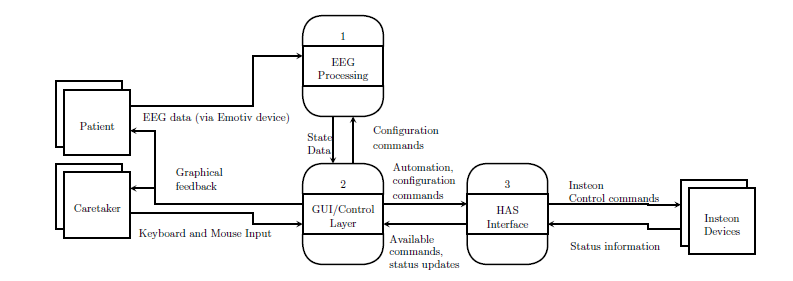
\includegraphics[width=0.8\linewidth]{level0DFD}
\captionof{figure}{Level 0 DFD of the main system components}
\end{center}

\end{multicols}
}

%----------------------------------------------------------------
% Machine Learning Methods
%-----------------------------------------------------------------
\headerbox{Machine Learning Model}{name=machinelearning,column=2,above=bottom, below=architecture}{

We trained a Naive Bayes Classifier by extracting 45 features from each of 6 electrodes in the EEG. The features were extracted by using a fast Fourier transform to convert the signal from each electrode from the time domain to frequency domain. Then we summed over different ranges corresponding to alpha (7-14Hz), beta (14-40Hz), delta (1-4Hz), theta (4-7Hz), and gamma (>40Hz). Once we summed these values for each electrode. We took the percentage difference between each range of each electrode on the right and the corresponding range of each electrode on the left. Since we monitored 6 electrodes, over 5 ranges, we get a total of 45 features. We sample these features over 1 second increments at 128Hz for 5 seconds to get the neutral state and then do it again for the active. Once these samples are used to create the classifier, we can classifier a given 1 second interval by giving the 45 features to the classifier and see what it returns. We do this for a rolling window and if at any point 4 consecutive windows correspond to the active state, we register an event. This is done to decrease the occurrence of false positives.

}

%----------------------------------------------------------------
% PROGRAM FLOW
%-----------------------------------------------------------------
\headerbox{Program Flow}{name=flow,column=0,row=1,below=objectives}{

At the application selection screen, the display cycles through the available
home automation system devices and the user decides which device they want to
interact with. When a device is chosen, the user is directed to the device's
interactive state screen, which presents available actions that can be
performed on that device. These actions include both simple changes, such as
toggling a light on or off, and also changes which require the user to enter
an integer, such as changing the television channel. From here, the user can
either change the state or return to the previous screen.

}

\headerbox{Program Flow Image}{name=flowimage,column = 1, above=bottom, below=introduction}{

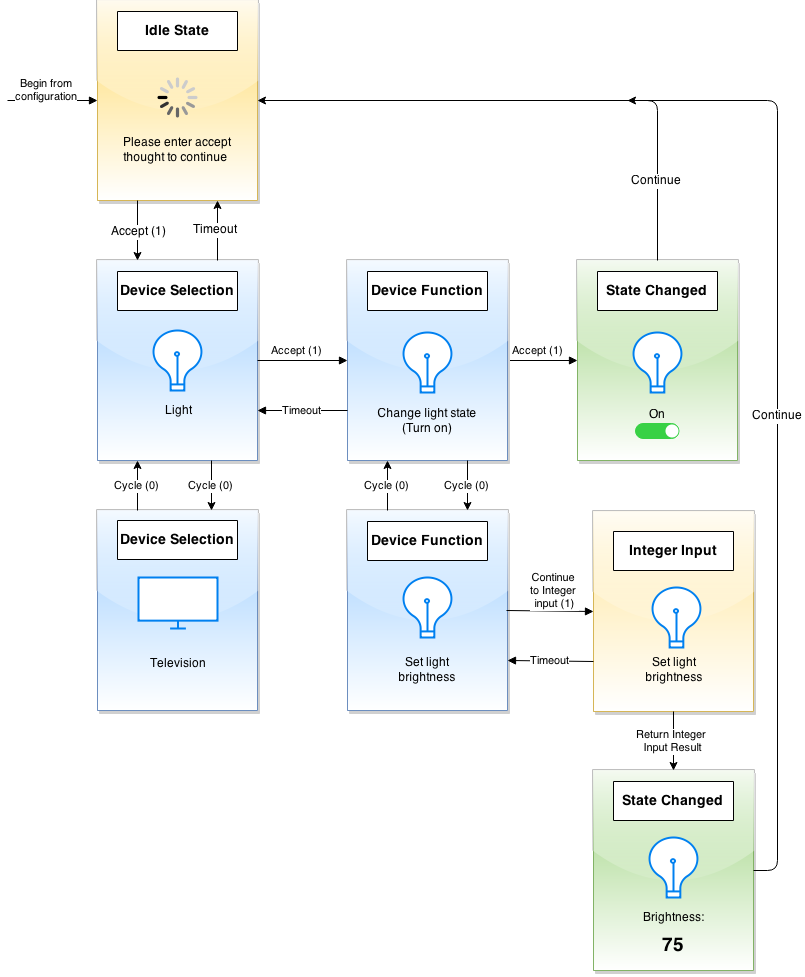
\includegraphics[width=0.9\linewidth]{ApplicationUI}
\captionof{figure}{General flow of the program}

}

%---------------------------------------------------------------------------------------- REFERENCES
%----------------------------------------------------------------------------------------

\headerbox{References}{name=references,column=0,above=bottom, below=flow}{
\begingroup
\renewcommand{\section}[2]{} % remove section header
\begin{thebibliography}{1}
    \bibitem{ALSsource} The ALS Association. (2014, October, 5). \textit{What
        is ALS?} [Online]. Available:
        \url{http://www.alsa.org/about-als/what-is-als.html}
 
    \bibitem{Emotiv} Emotiv, Inc. (2015, May, 5). \textit{Emotiv|EEG
        System} [Online]. Available: \url{http://emotiv.com/}
        
    \bibitem{Insteon} Insteon \textregistered. (2015, May, 5). \textit{Insteon} [Online]. Available: \url{http://www.insteon.com/}
\end{thebibliography}
\endgroup
}


%----------------------------------------------------------------------------------------
%	CONCLUSION
%----------------------------------------------------------------------------------------

\headerbox{Conclusion}{name=conclusion,column=3,span=1,row=0,below=architecture}{

%------------------------------------------------

\begin{itemize}\compresslist
\item ALS patients can achieve a huge quality of life improvement with a BCI by automating their house
\item The UI supports house automation through the input of the Emotiv Headset
\item We showed that the Insteon home automation system can be used without movement from the user using machine learning on EEG data
\end{itemize}
}

%----------------------------------------------------------------------------------------



%----------------------------------------------------------------------------------------
%	FUTURE RESEARCH
%----------------------------------------------------------------------------------------

\headerbox{Future Work}{name=futureresearch,column=3,span=1,below=conclusion}{ % This block is as tall as the references block

\begin{itemize}\compresslist
\item More devices can be controlled using the HAS (anything that uses an IR sensor,
    other Insteon devices)
\item The UI can be expanded to work with additional input types to ease use for users who are not fully locked-in
\item The machine learning signal-detection method can be refinedimproved
\end{itemize}
}

%----------------------------------------------------------------------------------------
%	CONTACT INFORMATION
%----------------------------------------------------------------------------------------

\headerbox{Contact Information}{name=contact,column=3,above=bottom, below=futureresearch}{ % This block is as tall as the references block

\begin{description}\compresslist
\item[Email] jgm55@drexel.edu
%\item[url] http://drexel.edu/cci/resources/current-students/undergraduate/senior-design-challenge/
\end{description}
}



\end{poster}

\end{document}
